\documentclass{ctexart}
\usepackage{graphicx}
\usepackage{amsmath}
\usepackage[a4paper,left=3.18cm,right=3.18cm,top=2.54cm,bottom=2.54cm]{geometry}

\title{工科数学分析数学实验报告}
\author{Leo}
\date{2022年12月10号}

\begin{document}
\maketitle
\section{实验一}
\subsection{实验题目}
用二分法求方程$4x^3-6x^2+3x-2=0$的近似解,要求误差不超过$10^{-5}$。
\subsection{实验目的及意义}
通过使用图形法求近似根,熟悉mathematica的函数运算指令,并对计算机求解方程近似解形成初步认识。
\subsection{程序设计}
\noindent f[x\_]:=4 x\^{} 3-6 x\^{}2+3 x-2;Plot[f[x],{x,1,2}]\\
Plot[f[x], \{x, 1.2, 1.3\}, PlotRange -> \{-0.1, 0.1\}]\\
Plot[f[x], \{x, 1.22, 1.23\}, PlotRange -> \{-0.01, 0.01\}]\\
Plot[f[x], \{x, 1.221, 1.222\}, PlotRange -> \{-0.001, 0.001\}]\\
Plot[f[x], \{x, 1.2211, 1.2212\}, PlotRange -> \{-0.0001, 0.0001\}]\\
\subsection{程序运行结果}
\noindent 首次输出函数f[x],可以看到该函数在1.2到1.4之间(不含端点)有一个根。
\begin{center}
	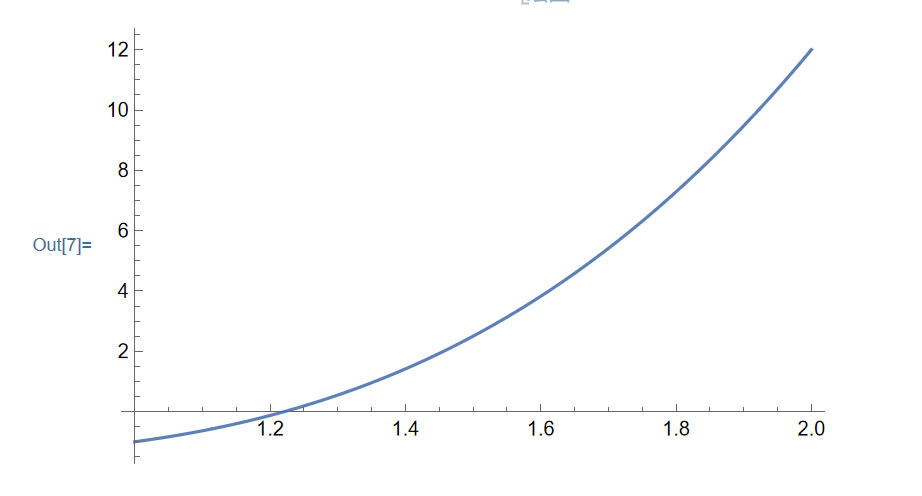
\includegraphics[scale=0.5]{1.png}\\
\end{center}
进一步约束绘图范围至[1.2,1.3]可以看到,根的近似度更高,在[1.22,1.23]之间:
\begin{center}
	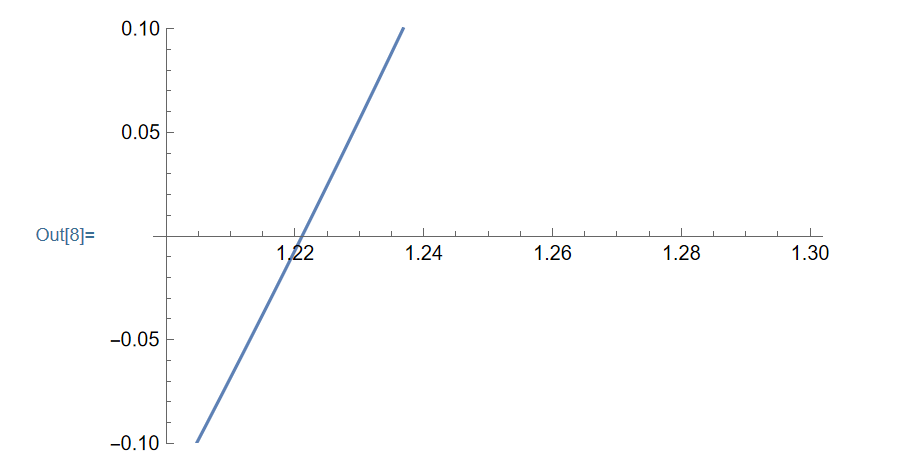
\includegraphics[scale=0.5]{2.png}\\
\end{center}
现在想更精确地得到根的近似值,于是一步步地缩小绘制范围,提高绘图精度,得到如下三幅图:
\begin{center}
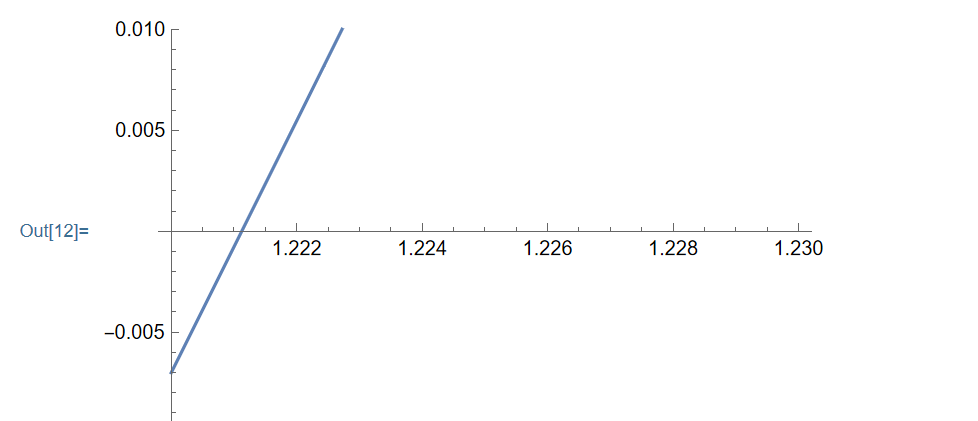
\includegraphics[scale=0.5]{3.png}\\
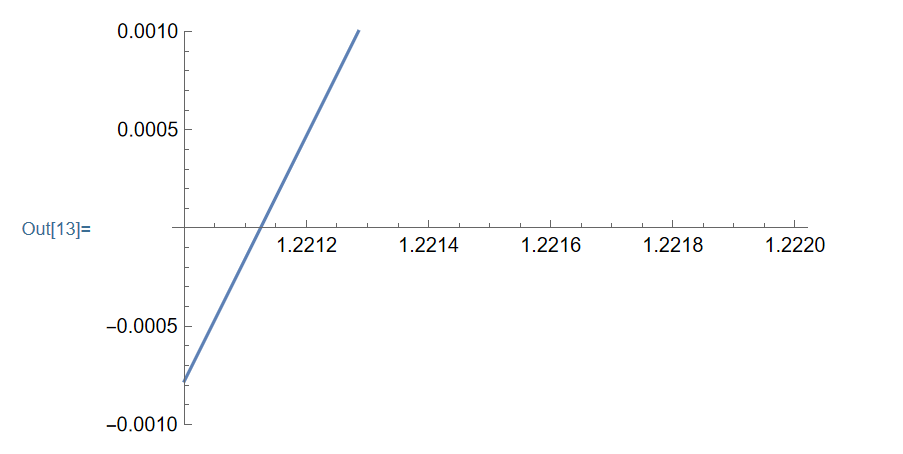
\includegraphics[scale=0.5]{4.png}\\
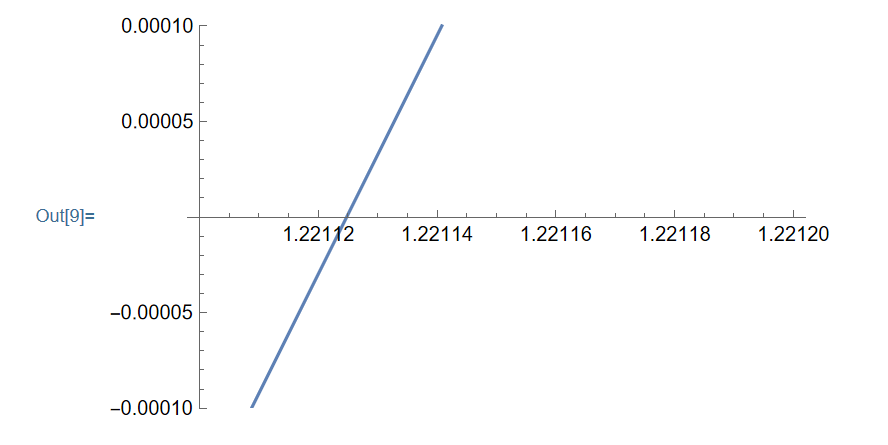
\includegraphics[scale=0.5]{5.png}\\
\end{center}

注意到此时的根落在[1.22112,1.22113]之间,取根的近似值为区间端点值1.22112,已经满足精度需要。故方程$4x^3-6x^2+3x-2=0$的近似解为x=1.22112,误差不超过$10^{-5}$。
\subsection{结果分析与讨论}
通过画图可以近似求得方程的根,并且可以通过一步步缩小绘图范围和提高绘图精度来得到理想精度的近似解。但是这种方法也有不足之处。比如,需要一次次根据上一次的作图结果确定下一次作图的取值范围,所以难以一次性得到理想精度的近似解。可能的解决办法有:使用Do循环,用牛顿迭代法或二分法求解。

\section{实验二}
\subsection{实验题目}
绘制点列图,观察重要极限:$\lim\limits_{n\to\infty}(1+\dfrac{1}{n})^n=e$.
\subsection{实验目的及意义}
直观感受散点函数逼近极限的过程,以便对重要极限$\lim\limits_{n\to\infty}(1+\dfrac{1}{n})^n=e$形成直观印象。
\subsection{程序设计}
an = \{(1 + 1/1)\^{}1, (1 + 1/2)\^{}2, (1 + 1/3)\^{}3\};\\
Do[an = Append[an, (1 + 1/i)\^{}i];\\
t = ListPlot[an, PlotRange -> \{2, 3\}, PlotStyle -> PointSize[0.015]];\\
Print[t], \{i, 4, 200\}]
\subsection{程序运行结果}
下面截取了n取不同值时的图像:
\begin{center}
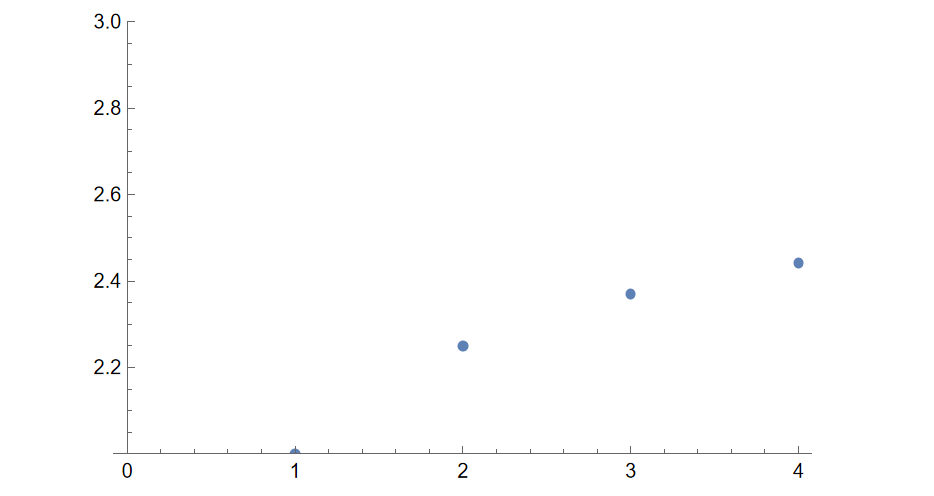
\includegraphics[scale=0.5]{6.png}
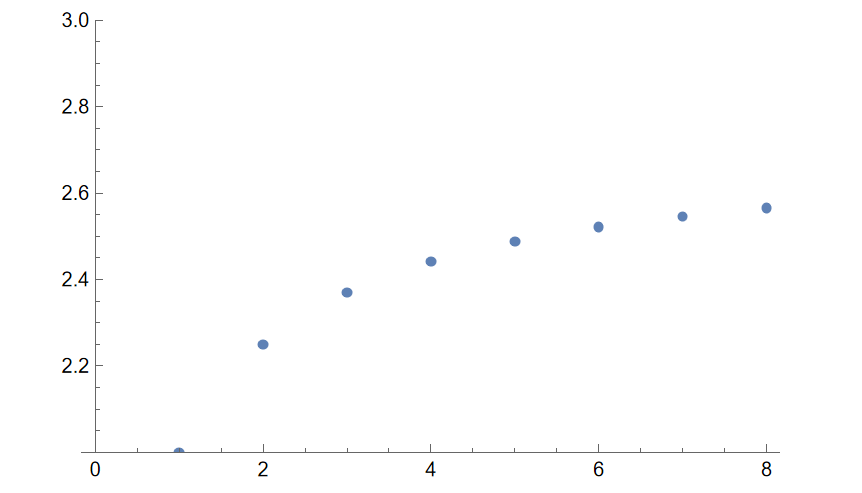
\includegraphics[scale=0.5]{7.png}
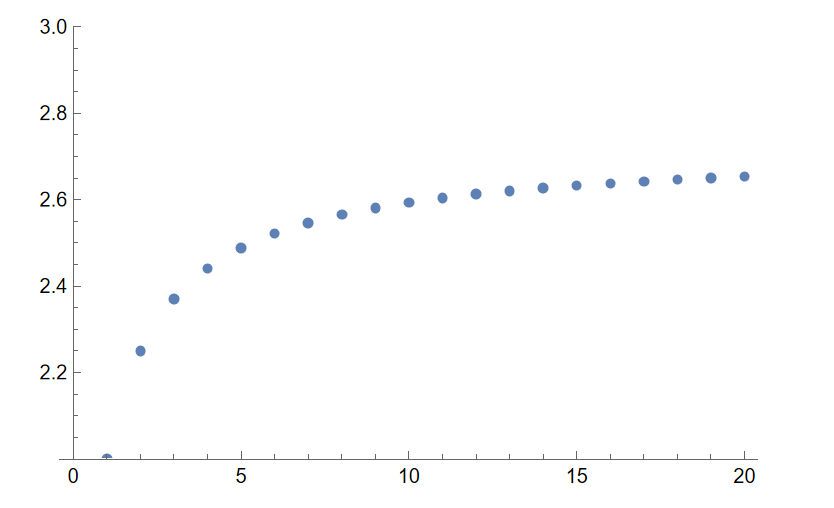
\includegraphics[scale=0.5]{8.png}
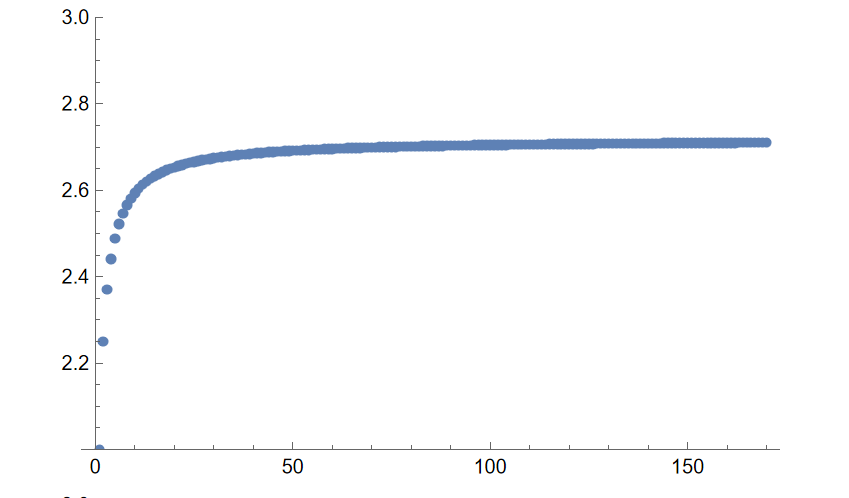
\includegraphics[scale=0.5]{9.png}
\end{center}

可以看到,当n很小(5以内)时,对应的函数值呈现明显的单增趋势,极限不明显。随着n的不断增大,函数值逐渐稳定于[2.6,2.6]区间。当n更大时,会发现函数值几乎稳定在2.7左右。
\subsection{结果分析与讨论}
由图像可以推测,$\lim\limits_{n\to\infty}(1+\dfrac{1}{n})^n$的值在2.7左右。由已有的极限知识可知,$\lim\limits_{n\to\infty}(1+\dfrac{1}{n})^n=e\approx 2.72$,实验现象与之吻合。
\section{实验三}
\subsection{实验题目}
已知函数$h(x)=x^5+x^4-5x^3-x^2+7x-3$,做出$h(x)$的函数图像,从图上观察极值点、驻点,并编程验证。
\subsection{实验目的及意义}
熟悉mathematica绘制函数全貌的功能,学会通过图像粗略估计函数的某些关键特征。加深对一元函数微分学以及函数性态的认识。
\subsection{程序设计}
\noindent h[x\_] = -3 + 7 x - x\^{}2 - 5 x\^{}3 + x\^{}4 + x\^{}5\\
Plot[h[x], \{x, 1, 2\}]\\
Plot[h[x], \{x, -3, 3\}, GridLines -> Automatic, Frame -> True, 
PlotStyle -> RGBColor[1, 0, 0]]\\
Plot[h'[x], \{x, -3, 3\}, GridLines -> Automatic, Frame -> True, 
PlotStyle -> RGBColor[1, 0, 0], PlotLabel -> "一阶导函数图像"]\\
Plot[h''[x], \{x, -3, 3\}, GridLines -> Automatic, Frame -> True, 
PlotStyle -> RGBColor[1, 0, 0], PlotLabel -> "二阶导函数图像"]\\
Solve[h'[x] == 0, x]\\
Solve[h''[x] == 0, x]\\
\subsection{程序运行结果}
当运行到Plot[h[x], \{x, 1, 2\}]时,发现函数明显没有展现出全貌,于是使用带网格线和边框的绘图命令:\\Plot[h[x], \{x, -3, 3\}, GridLines -> Automatic, Frame -> True, 
PlotStyle -> RGBColor[1, 0, 0]]\\
可以看到,函数整体形态如下:
\begin{center}
	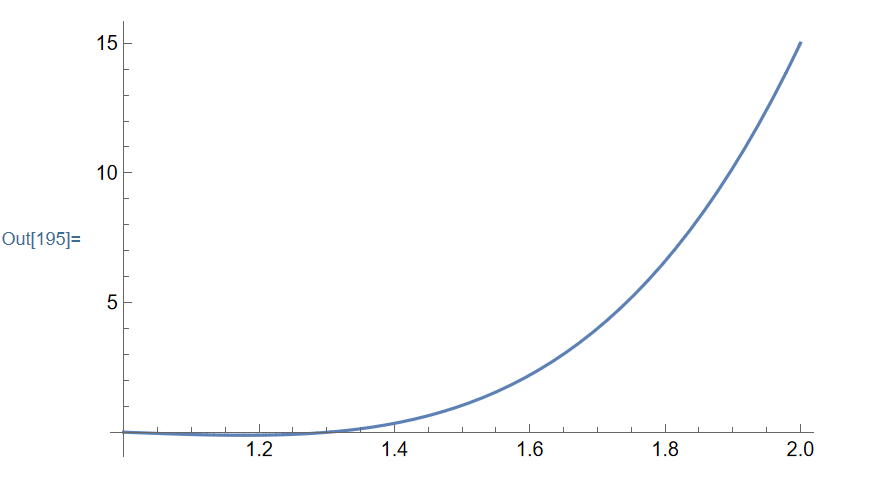
\includegraphics[scale=0.5]{10.png}
\end{center}
此时可以粗略判断,函数在-2,-0.7,0.7,1.2附近取到极值,没有驻点。那么是否确实如此呢?接下来的命令:\\Plot[h'[x], \{x, -3, 3\}, GridLines -> Automatic, Frame -> True, 
PlotStyle -> RGBColor[1, 0, 0], PlotLabel -> "一阶导函数图像"]\\
Plot[h''[x], \{x, -3, 3\}, GridLines -> Automatic, Frame -> True, 
PlotStyle -> RGBColor[1, 0, 0], PlotLabel -> "二阶导函数图像"]\\
绘制了h[x]一阶导函数和二阶导函数的图像,通过它们的零点来判断h(x)的性态:
\begin{center}
	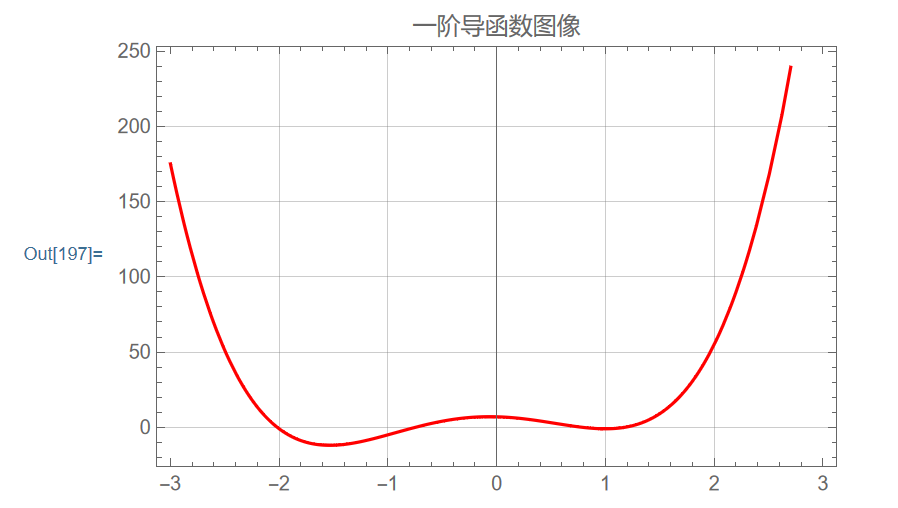
\includegraphics[scale=0.5]{一阶导函数.png}
	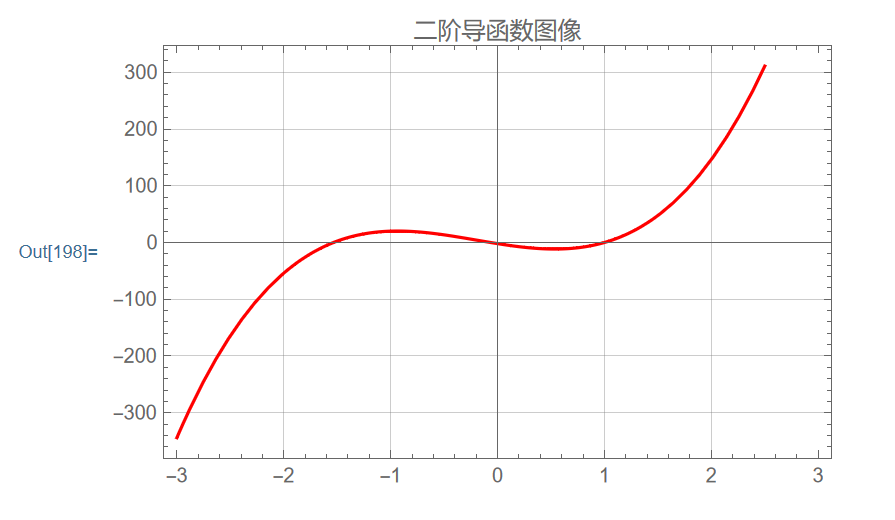
\includegraphics[scale=0.5]{二阶导函数.png}
\end{center}
可以看到,一阶导函数和二阶导函数已经展现出来,对应h(x)本身,结合导函数零点与函数单调性的关系可知,上文的估计大体正确。更进一步,此时若想要求得函数较为精确的极值点,则可以使用methematica的解方程功能:\\
Solve[h'[x] == 0, x]\\
Solve[h''[x] == 0, x]\\
分别求解一阶导函数和二阶导函数等于0时的x值,如下图所示:
\begin{center}
	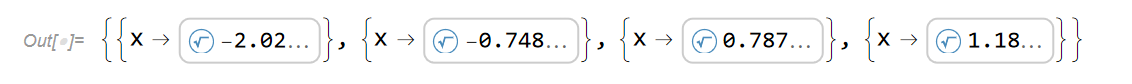
\includegraphics[scale=0.5]{一阶导函数的解.png}
	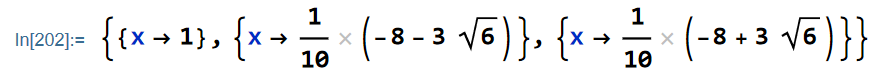
\includegraphics[scale=0.5]{二阶导函数的解.png}
\end{center}
至此,我们已经较为精确地解得了h(x)的极值点。\\
注:如果想要对一阶导函数等于0的方程求数值解,可采用以下代码:\\
\begin{center}
	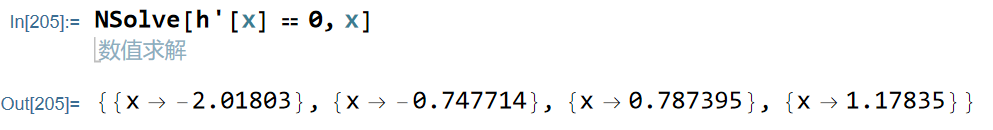
\includegraphics[scale=0.5]{注解.png}
\end{center}
\subsection{结果分析与讨论}
通过以上案例分析可得,函数的极值点,驻点,单调性和其一阶导函数,二阶导函数等有密切关系。利用mathematica,不仅可以使用作图命令得到较为直观的印象,还可以使用解方程功能,求得方程较为精确的近似解。

\end{document}